\documentclass{llncs}
\usepackage[utf8]{inputenc}
\usepackage{graphicx}
\usepackage{color}
\usepackage{url}
\usepackage[spanish]{babel}
\usepackage{epstopdf}

\begin{document}

%%%%%%%%%%%%%%%%%%%%%%%%%%%%%%%   TITLE   %%%%%%%%%%%%%%%%%%%%%%%%%%%%%%%

\title{Progamer: aprendiendo a programar usando videojuegos como metáfora para visualización de código.}

%%%%%%%%%%%%%%%%%%%%%%%%%%%%%%%   AUTHORS   %%%%%%%%%%%%%%%%%%%%%%%%%%%%%%%

\author{J.J. Asensio, A.M. Mora, \\P. García-Sánchez, J.J. Merelo, P.A. Castillo}
\authorrunning{J.J. Asensio et al.}

\institute{
Departamento de Arquitectura y Tecnología de Computadores. \\
Escuela Técnica Superior de Ingenierías Informática y de Telecomunicación. \\
Universidad de Granada, España \\
\email{\{asensio, amorag, pablogarcia, jmerelo, pacv\}@ugr.es }  
}
% la dirección de pablo es pgarcia y tú no sé si tienes - JJ
\maketitle
%
%%%%%%%%%%%%%%%%%%%%%%%%%%%%%%%%%   ABSTRACT   %%%%%%%%%%%%%%%%%%%%%%%%%%%%%%%%%
%
\begin{abstract} 
Las herramientas de visualización de software a nivel de componente
pueden ser utilizadas durante el desarrollo y mantenimiento del mismo
para detectar y visualizar posibles defectos. Estas herramientas
suelen ser diseñadas como complementos en los entornos de programación y
muestran las relaciones entre las clases permitiendo navegar también
visualmente a través del software. Sin embargo también pueden ser
útiles durante el aprendizaje de los conceptos básicos de
programación. En este sentido es necesario dotar a las herramientas de
características adicionales que faciliten este aprendizaje. Para tal
fin, este trabajo explora el uso de metáforas inspiradas en técnicas de gamificación a través de la visualización de código presentando la herramienta \emph{Progamer}: un
complemento de Eclipse para visualización de código Java a nivel de método,
basado en mapa, que utiliza un videojuego de plataformas como metáfora basada en agente.
\end{abstract}


%
%%%%%%%%%%%%%%%%%%%%%%%%%%%%%%%   INTRODUCTION   %%%%%%%%%%%%%%%%%%%%%%%%%%%%%%%
%
\section{Introducción}
\label{sec:intro}
La visualización de software es un amplio campo de investigación que cubre las diferentes técnicas de asistencia empleadas en las actividades de ingeniería del software, tales como especificación, diseño, programación, test, mantenimiento, ingeniería inversa o re-ingeniería. Los métodos empleados habitualmente representan gráficamente (en 2D o 3D), de forma estática o dinámica (con animaciones), información relacionada con la estructura, tamaño, historia o comportamiento del software. El objetivo es facilitar la comprensión de diferentes aspectos del sistema \cite{baecker1988enhancing}. Esta visualización también permite analizar la complejidad de un sistema y detectar anomalías o defectos de calidad en el software, lo que facilita su evolución \cite{softwarevisualization}. La visualización de programas concretamente trata de representar gráficamente el código o los datos. 

A nivel educativo intuitivamente se han empleados diferentes técnicas de visualización de software para el aprendizaje de los conceptos de programación y algoritmos básicos \cite{urquiza2009survey}. Sin embargo, no está claro que las técnicas utilizadas de por sí mejoren directamente el aprendizaje si no son complementadas con otras prácticas pedagógicas \cite{naps2002exploring}. En este sentido es necesario proveer de nuevas formas de visualización que tengan en cuenta o encajen mejor con los métodos de enseñanza empleados, entre los cuales podemos destacar el uso de técnicas de \emph{gamificación} \cite{salen2011quest}.

Para representar la estructura de un programa escrito en un lenguaje orientado a objetos, el enfoque consiste en visualizar las dependencias existentes entre las diferentes clases. Estas dependencias puede ser modeladas como un grafo por lo que la visualización siguiendo dicha estructura resulta muy adecuada. El software a un nivel más básico, es decir, a nivel de método, puede ser también representado de esta forma mediante un diagrama de flujo, el cual estará compuesto por nodos y aristas.

Sin embargo, el código de un método cumple además con las reglas sintácticas del lenguaje, por lo que también puede ser representado mediante su árbol sintáctico abstracto. En este árbol los nodos representan los diferentes elementos del lenguaje utilizados y las aristas su relación de inclusión (por ejemplo el nodo IF tiene como nodos hijos la parte THEN y la parte ELSE, cada una con sus propios nodos hijos). A diferencia del diagrama de flujo, la visualización en forma de árbol es mucho más flexible. Por ejemplo, la jerarquía de un árbol puede ser visualizada mediante un mapa 2D sin necesidad de utilizar flechas \cite{softwarevisualization}.


\begin{figure}[ht]
\begin{center}
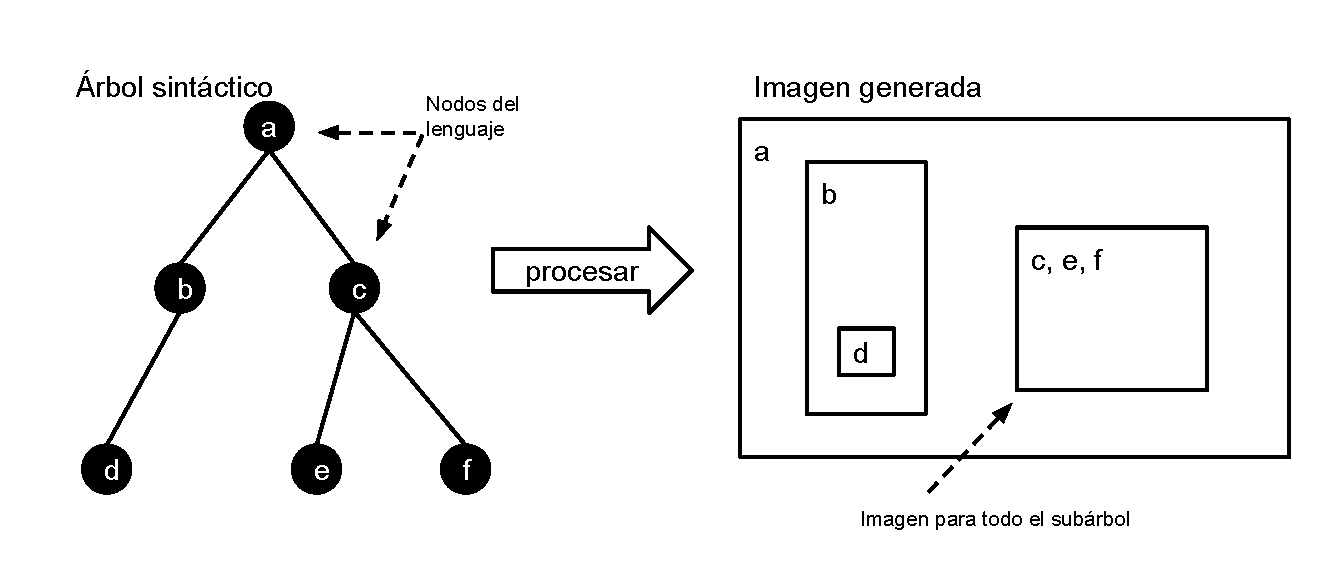
\includegraphics[scale=0.5]{images/arbol-mapa.pdf}
\caption{La imagen está compuesta por los gráficos generados para los elementos a, b, c y d. Los nodos e y f comparten representación con el nodo c. La disposición de unas imágenes dentro de otras sigue unas reglas de composición determinadas que dependen del tipo de nodo contenedor.
\label{fig:arbolmapa}}
\end{center}
\end{figure}

Por otra parte, la representación en forma de mapa, permite visualizar los diferentes nodos del lenguaje empleados con un nivel de precisión arbitrario. Es decir, si por ejemplo no queremos visualizar detalles de una expresión, podemos visualizarla como un determinado objeto gráfico del mapa sin mostrar en su interior los elementos que la componen (ver figura \ref{fig:arbolmapa}).

Además, el establecimiento de reglas adecuadas para la representación de los diferentes nodos del lenguaje y su composición interna (nodos hijos) nos permite proyectar de manera flexible, pero completamente objetiva el código del programa sobre una imagen representativa. Esta flexibilidad creativa ofrecida por las reglas de composición, habilita la cosificación o materialización de metáforas \cite{travers1996programming} en imágenes que pueden ser generadas automáticamente según qué aspecto del código se quiera reflejar con ellas. De esta forma es posible visualizar un mismo programa, usando diferentes metáforas, atendiendo al contexto de utilidad o asistencia deseada, como puede ser mantenimiento, evolución, tests, calidad, navegación, etc.

En el caso del aprendizaje interesa que la metáfora utilizada resulte atractiva para el estudiante. Para ello, este trabajo propone utilizar el escenario de un videojuego de plataformas como metáfora del árbol sintáctico abstracto del programa. Esta visualización encaja bien dentro de las técnicas de gamificación en educación como las empleadas en \cite{kumar2012gamification}, donde se transforma en juego y competición todo el contexto de enseñanza de una asignatura de programación. 

Por otra parte, nuestro enfoque resulta ser también una visualización dinámica, puesto que la metáfora empleada es animada y existe una asociación directa entre ambos contextos semánticos, es decir, el protagonista del videojuego corre por el mapa y el ordenador ejecuta (corre) el programa. 

Esta metáfora también permite la creación de \emph{juegos serios} donde la mecánica en realidad sería muy distinta a la del videojuego original, pues se trataría de diseñar un mapa (programa) aplicando ciertas restricciones que al ser recorrido (ejecutado) resuelva un problema dado. Hasta donde sabemos, no existe ninguna herramienta similar ni trabajos relacionados que apliquen esta técnica.

Para la implementación de una herramienta de visualización dinámica de estas características se ha utilizado el lenguaje Java y el entorno de desarrollo integrado (IDE) Eclipse. 

El resto de este trabajo está organizado de la siguiente forma: en la sección \ref{sec:background} se explora el contexto taxonómico, se discute el concepto de legibilidad del código y su relación con algunas herramientas existentes para el aprendizaje de programación orientada a objetos. Además se describen las técnicas de gamificación y la importancia de su papel en la metáfora conceptual propuesta. En la sección \ref{sec:proposal} se describe la herramienta presentada concretando sus características. En la sección \ref{sec:details} se detallan los principales aspectos de la implementación. Por último en la sección \ref{sec:conclusions} se establecen las conclusiones obtenidas y la continuación de este trabajo. 

%
%%%%%%%%%%%%%%%%%%%%%%%%%%%%%%%   BACKGROUND  %%%%%%%%%%%%%%%%%%%%%%%%%%%%%%%
%
\section{Contexto}
\label{sec:background}
%----------------------------------------------------------------------------
\subsection{Metáfora conceptual}

La idea de utilizar metáforas para la representación y comprensión de conceptos abstractos es fundamental durante el aprendizaje. El término ``metáfora" que se usa aquí va más allá del sentido lingüístico habitual utilizado como recurso literario. En realidad se refiere al modelo metafórico por el cual se estructura el conocimiento de un dominio objetivo mediante la asociación al mismo de conceptos y relaciones de otro dominio origen existente con el que ya se está familiarizado. 

Las metáforas son empleadas, por ejemplo dentro del campo de las matemáticas, con las que se enseña todo tipo de conceptos. Algunos símbolos matemáticos, como por ejemplo, los paréntesis, pueden ser interpretados como metáforas, en el sentido de que encierran explícitamente un determinado contenido. Podríamos decir que su uso como símbolo posee un significado visual añadido. Existe sin embargo un inconveniente cuando se hace un uso intensivo de estos símbolos ya que pierden su capacidad explicativa, como se observa a continuación en el siguiente programa escrito en Lisp:

\begin{verbatim}
(defun factorial (n) (if (<= n 1) 1 (* n (factorial (- n 1)))))
\end{verbatim}

Otro ejemplo es el uso de flechas para indicar transiciones de un punto a otro. Al igual que con los paréntesis, al aumentar el número de flechas, aumenta la dificultad de comprensión del diagrama. Además, al ser utilizadas frecuentemente en diferentes contextos y con diferente significado, las flechas adquieren un cierto nivel de abstracción, que devalúa todavía más su capacidad aclaratoria. 

Con estos ejemplos se intenta ilustrar la importancia y necesidad de encontrar representaciones visuales concretas que faciliten la comprensión, documentación y el aprendizaje de forma específica según el tipo de conceptos que se utilizan en programación y que además puedan ser generadas automáticamente a partir del código. En \cite{travers1996programming} se introduce el concepto de metáfora basada en agente, el cual tiene propiedades antropomórficas como autonomía, propósito y estado emocional que se pueden corresponder con objetos del dominio de la programación.

Para el diseño de metáforas útiles en programación, es necesario conseguir un compromiso adecuado entre la abstracción asociada a los elementos visuales y su analogía semántica con el elemento representado. Además resulta también útil hacer que estas representaciones sean atractivas para el estudiante durante el aprendizaje. 


%----------------------------------------------------------------------------
\subsection{Contexto taxonómico del uso de gráficos en programación}
\label{subsec:taxonomy}
Los sistemas que usan gráficos para programar, depurar y entender la computación en general han proliferado desde el inicio de la informática. La idea de hacer más accesible la programación a cualquier tipo de usuario ha demandado la utilización de gráficos o lenguajes visuales para la confección de programas. De igual forma el uso de gráficos facilita la comprensión de lo que el programa hace así como su depuración cuando se enseña a programar a los estudiantes. 

En este contexto muchas veces los términos utilizados para el uso de gráficos son a menudo informales o confusos. En 1990 Myers \cite{myers1990taxonomies} estableció una taxonomía formal para los diferentes sistemas gráficos utilizados en aquel entonces y que continúa siendo válida. De esta forma establece la visualización de un programa como el uso de gráficos que ilustran algún aspecto del mismo o de su ejecución. En la figura \ref{fig:flowchart} se muestra un ejemplo de visualización de código de forma estática. En concreto la visualización de un programa se clasifica según se visualiza el código, los datos o el algoritmo. Tal visualización además puede ser estática o dinámica dependiendo de si existe algún tipo de animación mientras se ejecuta el programa \cite{urquiza2009survey}. 

\begin{figure}[ht]
\begin{center}
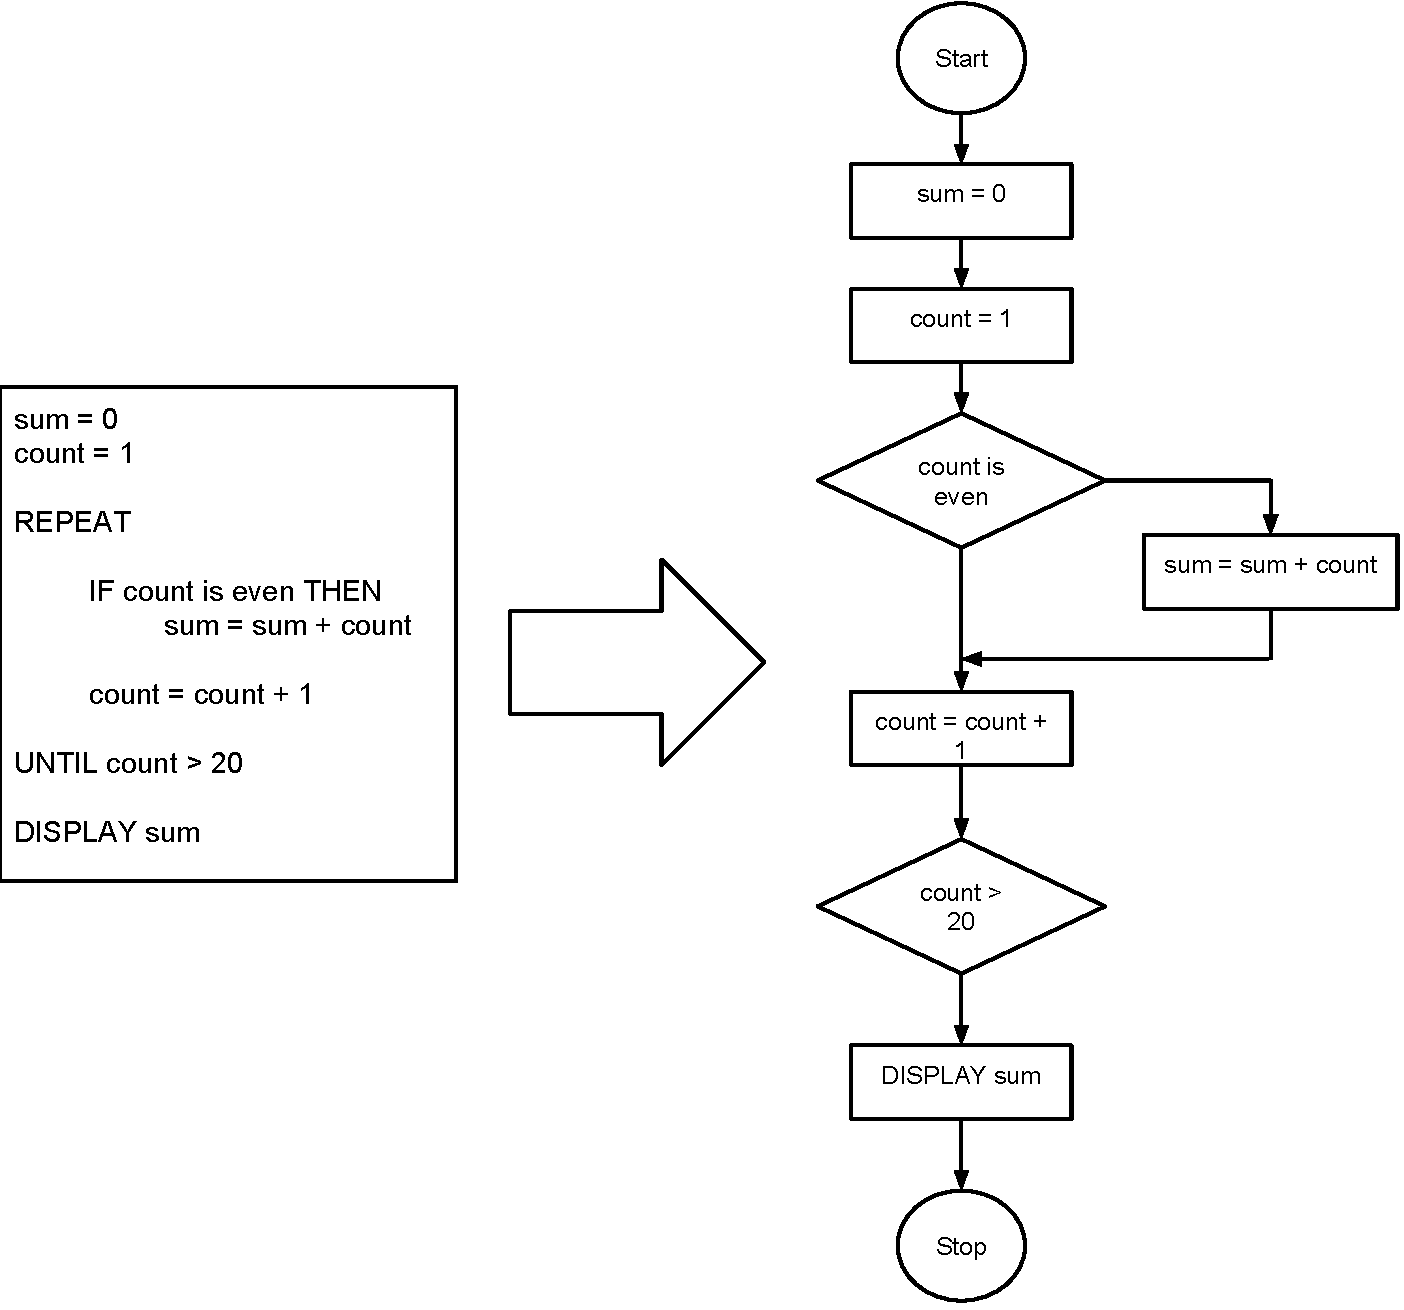
\includegraphics[scale=0.45]{images/flowchart2.pdf}
\caption{El diagrama de flujo visualiza el código asociado de forma estática.
\label{fig:flowchart}}
\end{center}
\end{figure}

La justificación se fundamenta en que el sistema visual humano está optimizado para procesar información multidimensional mientras que la programación convencional, sin embargo, es representada como un texto unidimensional. En este sentido, la capacidad del código de ser entendido por un humano, es decir, su legibilidad, es discutida a continuación destacando la visualización de código empleada en algunas herramientas que se utilizan para enseñar la programación. En tales ejemplos se pone de manifiesto la necesidad de exploración y explotación de nuevas metáforas que, aplicadas a un contexto puramente computacional, sean adecuadamente flexibles para expresar, resumir, documentar y comprender mejor el código. 

%----------------------------------------------------------------------------
\subsection{Legibilidad}
\label{subsec:readability}
A menudo se hace una analogía entre el texto de un programa y el texto narrativo. La legibilidad en este sentido, como concepto, es decir, la capacidad de que algo sea leído por un humano, es una idea general muy amplia. El término ``leído'' implica todas las fases del procesamiento del lenguaje a fin de que el significado sea entendido por el lector. Con esta definición en mente vemos claramente diferencias sustanciales entre la legibilidad de un texto narrativo y el código de un programa. 

La legibilidad del texto narrativo depende de la historia que se cuenta y de cómo el lector puede representar, mediante su imaginación, el significado natural de esta historia conforme a su experiencia. Si la historia es confusa o carece de sentido, el texto es poco legible. Sin embargo, es posible que la historia tenga pleno sentido y sea clara y que el texto siga siendo poco legible, por ejemplo, imaginemos un niño leyendo un artículo científico. En este caso la experiencia del lector es el factor predominante. 

Si aplicamos esta misma idea al texto de un programa, resulta obvio que la ``historia'' que expresa el programa poco tiene que ver con la experiencia del lector. Su significado existe en un contexto computacional, matemático-lógico completamente distinto, generalmente abstracto, y por tanto contrapuesto, al mundo real del lector. Para que el texto del programa sea legible por tanto sólo hay dos opciones: 

\begin{itemize}
\item o bien forzamos el contexto semántico del programa para que se adecue a la experiencia natural del lector, 
\item o bien reforzamos la experiencia del lector en el contexto de la programación. 
\end{itemize}

\subsubsection{La semántica del mensaje.}
\label{subsec:message}

En el primer caso se intenta conseguir que el lector se introduzca en la programación partiendo de su experiencia natural. Su alcance, si bien importante, está limitado a la generación de programas cuya salida es multimedia y presenta alguna historia interactiva. El código usado para este fin concreto se limita a un conjunto específico de instrucciones. Incluso así, este código puede no ser legible hasta que finalmente se ejecute. 

Algunas herramientas que utilizan este enfoque son:
\begin{itemize}
\item {\em Squeak Etoys}: Es un IDE dirigido a niños y un lenguaje de programación basado en prototipos y orientado a objetos \cite{etoysOnline}. Dirigido e inspirado por Alan Kay para promover y mejorar el constructivismo. Los principales influyentes en esta herramienta son Seymour Papert y el lenguaje Logo. La figura \ref{fig:etoys} muestra un programa de ejemplo.


\begin{figure}[ht]
\begin{center}
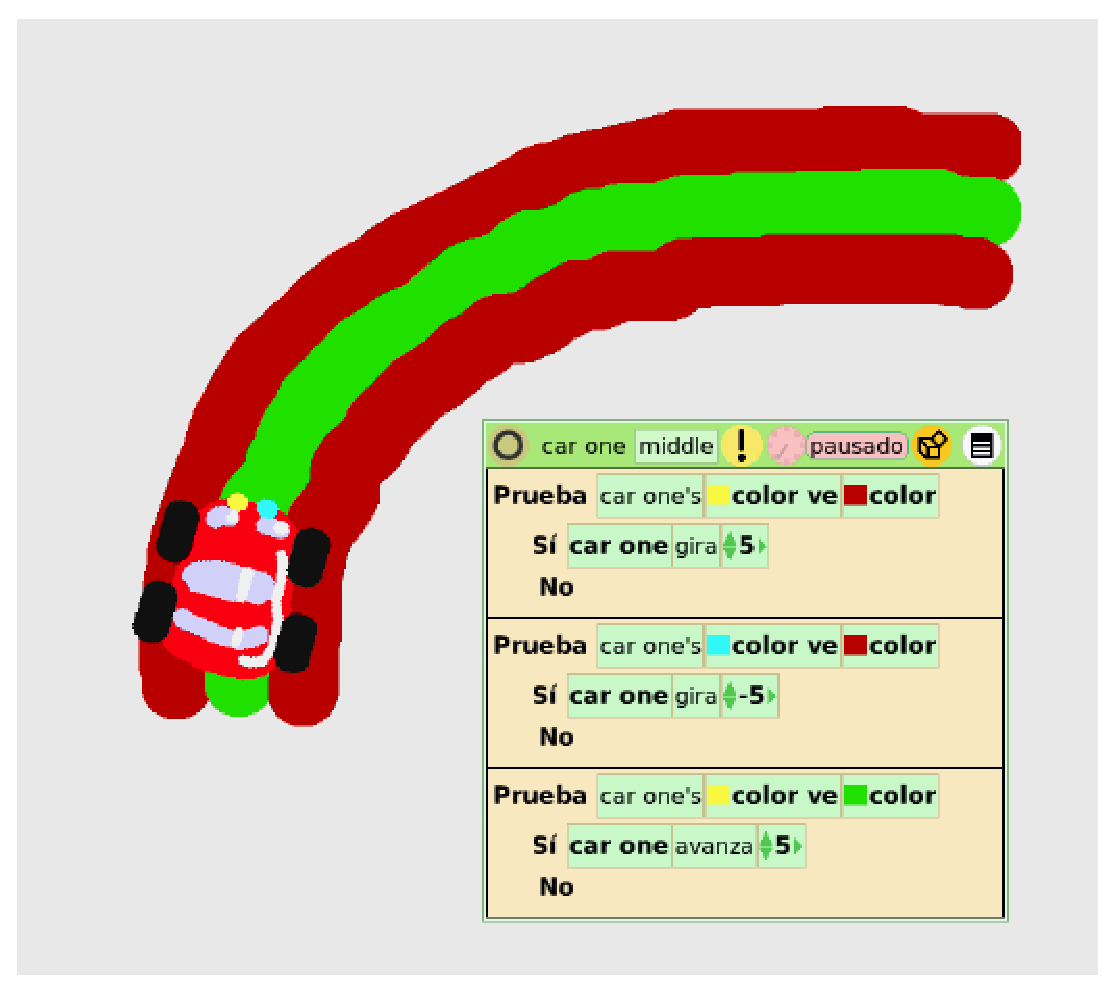
\includegraphics[scale=0.4]{images/etoys.eps}
\caption{Un programa diseñado en Etoys para controlar un coche sigue-línea. Los sentencias condicionales se apilan secuencialmente como rectángulos.
\label{fig:etoys}}
\end{center}
\end{figure}

\item {\em Alice}: Alice \cite{AliceOnline} es un lenguaje de programación educativo libre y abierto orientado a objetos con un IDE programado en Java. Utiliza un entorno sencillo basado en arrastrar y soltar para crear animaciones mediante modelos 3D. Este software fue desarrollado por los investigadores de la Universidad Carnegie Mellon, entre los que destaca Randy Pausch. En la figura \ref{fig:alice} podemos ver el aspecto típico que tiene el código.

\begin{figure}[ht]
\begin{center}
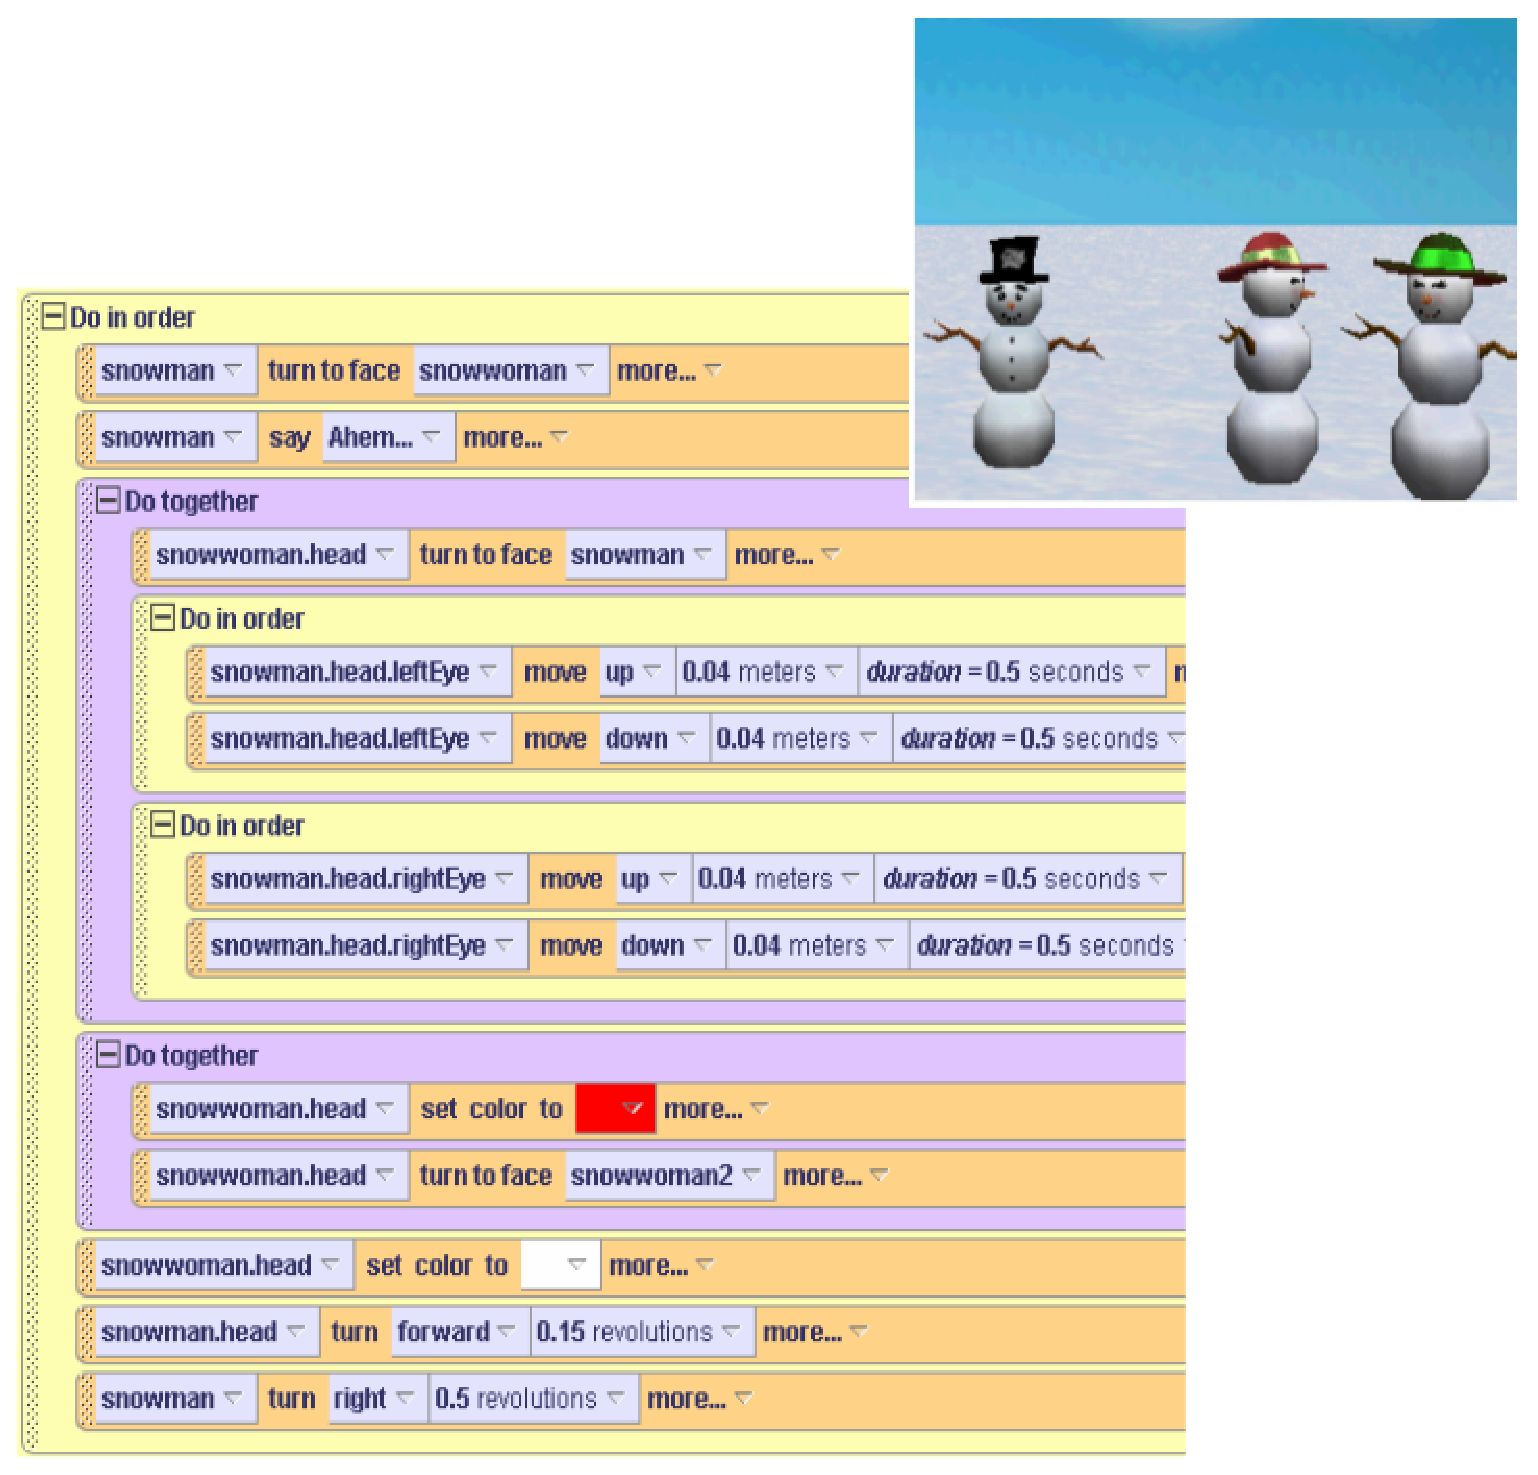
\includegraphics[scale=0.4]{images/alice.eps}
\caption{El código en Alice es empaquetado en cajas desplegables de distinto color según se ejecutan en serie o en paralelo las instrucciones contenidas.
\label{fig:alice}}
\end{center}
\end{figure}

\item {\em Scratch}: Es un entorno de programación online \cite{ScatchOnline} que facilita el aprendizaje autónomo. Fue desarrollado por el ``the Lifelong Kindergarten group'' en el Media Lab del MIT (Massachussets Institute of Tecnology) por un equipo dirigido por Mitchel Resnick y apareció por primera vez en el verano de 2007 \cite{resnick2009scratch}. La figura \ref{fig:scratch} muestra un programa de ejemplo. Los elementos de programación son representados como bloques de distinto color que encajan entre sí.
\end{itemize}


\begin{figure}[ht]
\begin{center}
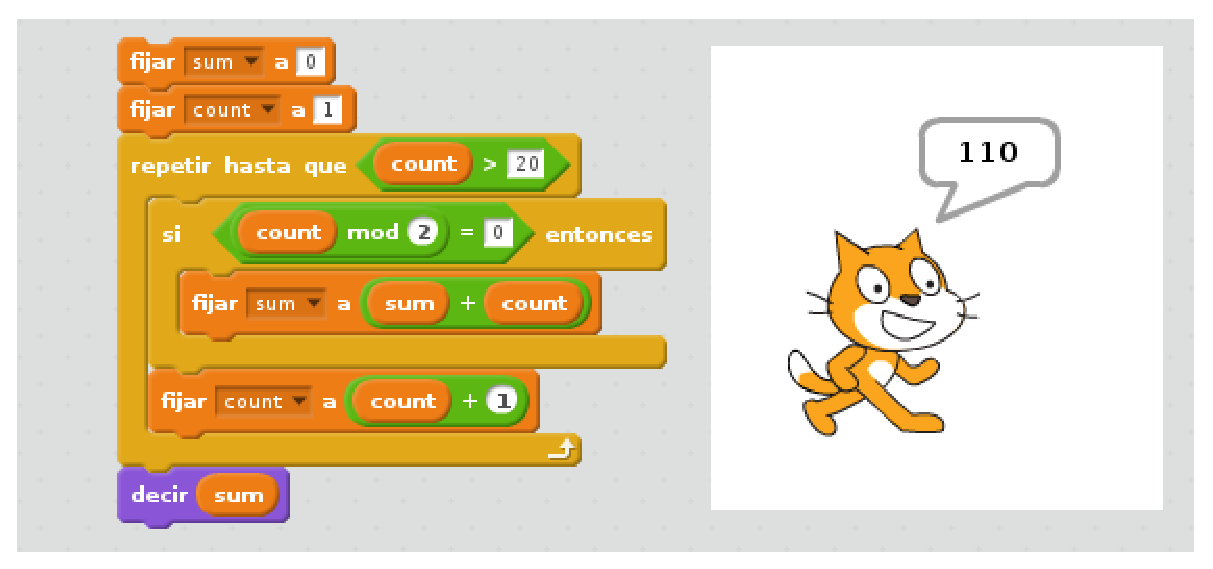
\includegraphics[scale=0.4]{images/scratch.eps}
\caption{El mismo programa de la figura \ref{fig:flowchart} diseñado con Scratch. Las instrucciones son visualizadas como bloques encajables. 
\label{fig:scratch}}
\end{center}
\end{figure}


\subsubsection{La experiencia del lector.}
\label{subsec:reader}

El segundo caso por otra parte, tiene un alcance mucho más amplio y por tanto más difícil de conseguir. Es necesario trabajar multitud de conceptos como los algebraicos, lógicos y matemáticos desde edades tempranas. Además, la naturaleza abstracta de estos conceptos dificulta su propia representación visual. En este sentido, algunos conceptos son más susceptibles que otros de ser visualizados, como por ejemplo los conjuntos y sus operaciones, las funciones matemáticas, o los vectores, son más fáciles de visualizar que otros como la probabilidad, las derivadas o las diferentes partículas subatómicas. Esta visualización es importante durante el aprendizaje.

Como vemos, el concepto general de legibilidad en el ámbito de la programación no está claro. El motivo principal es claramente la confusión de no tener en cuenta que el verdadero lector efectivo del texto de un programa no es una persona, sino una máquina. 

Desde este enfoque más amplio, es posible arrojar más luz sobre la comprensión de los procesos subyacentes en el aprendizaje de la programación. De aquí la importancia de la documentación del código \cite{tenny1988program}, a menudo descuidada. Es necesario abordar una automatización de generación de documentación legible entendiendo esta documentación, no sólo como un contenido añadido al programa, sino más bien como una característica intrínseca durante la generación y depuración del programa \cite{baecker1988enhancing}. En este paradigma el programador escribe y tanto el humano como la máquina pueden leer. Puesto que la máquina y el ser humano leen de forma diferente es necesario proveer al programador de diferentes herramientas para generar paralelamente al código y de forma automática, distintas representaciones significativas (de dominios conocidos) para sí mismo y para otras personas. Estas herramientas pueden ser especialmente efectivas durante el aprendizaje si se aplican metáforas donde el dominio de origen asociado a tales representaciones resulte atractivo para el estudiante.

Para este fin, a continuación se exploran las técnicas de gamificación y algunos ejemplos en el contexto educativo. La idea es tomar prestada la experiencia de la persona al jugar a videojuegos para hacer más intuitivo y atractivo el proceso de aprendizaje del uso de estructuras básicas de control en lenguajes imperativos. 


%----------------------------------------------------------------------------
\subsection{Gamificación}
\label{subsec:gamification}

La gamificación consiste en el uso de mecánicas de juego o pensamiento de juego en un contexto ajeno al juego, con el fin de conseguir determinados objetivos. Esta técnica aprovecha la predisposición psicológica del humano a participar en juegos. Las técnicas utilizadas consisten básicamente en tres tipos:
\begin{itemize}
\item {\em A)} Ofrecer recompensas por la realización de las tareas. 
\item {\em B)} Aprovechar la competitividad, haciendo visibles las recompensas entre los jugadores.
\item {\em C)} Hacer más atractivas tareas ya existentes que normalmente pueden ser aburridas. 
\end{itemize}

El campo de la educación presenta un gran potencial de crecimiento para la gamificación \cite{lee2011gamification}, existiendo multitud de ejemplos de uso de gamificación para el aprendizaje. Quizá el más llamativo es la escuela neoyorquina Quest to Learn \cite{salen2011quest}, donde todo el proceso de aprendizaje está dirigido al juego. 

Un ejemplo concreto de gamificación aplicado al aprendizaje de programación es Codecademy \cite{codecademy}. Esta plataforma online interactiva ofrece clases gratuitas de programación con diferentes lenguajes. La técnica de gamificación usada en este contexto es la de recompensar y motivar la competitividad de los estudiantes, es decir las técnicas A y B. 

%ANTARES: Si quieres citar más, tienes CodeAvengers que es de los más populares junto a CodeSchool con su Rails for Zombies o TryRuby.

En relación a la tercera técnica enumerada C, entre los ejemplos existentes podemos destacar ParticleQuest, el cual trata de enseñar a los estudiantes de física las partículas subatómicas. La metáfora consiste en identificar las partículas subatómicas como personajes enemigos de un videojuego tipo RPG (Role-Playing Game). Las diferentes características de cada partícula identifican las habilidades y morfología de los diferentes personajes. 

\begin{figure}[ht]
\begin{center}
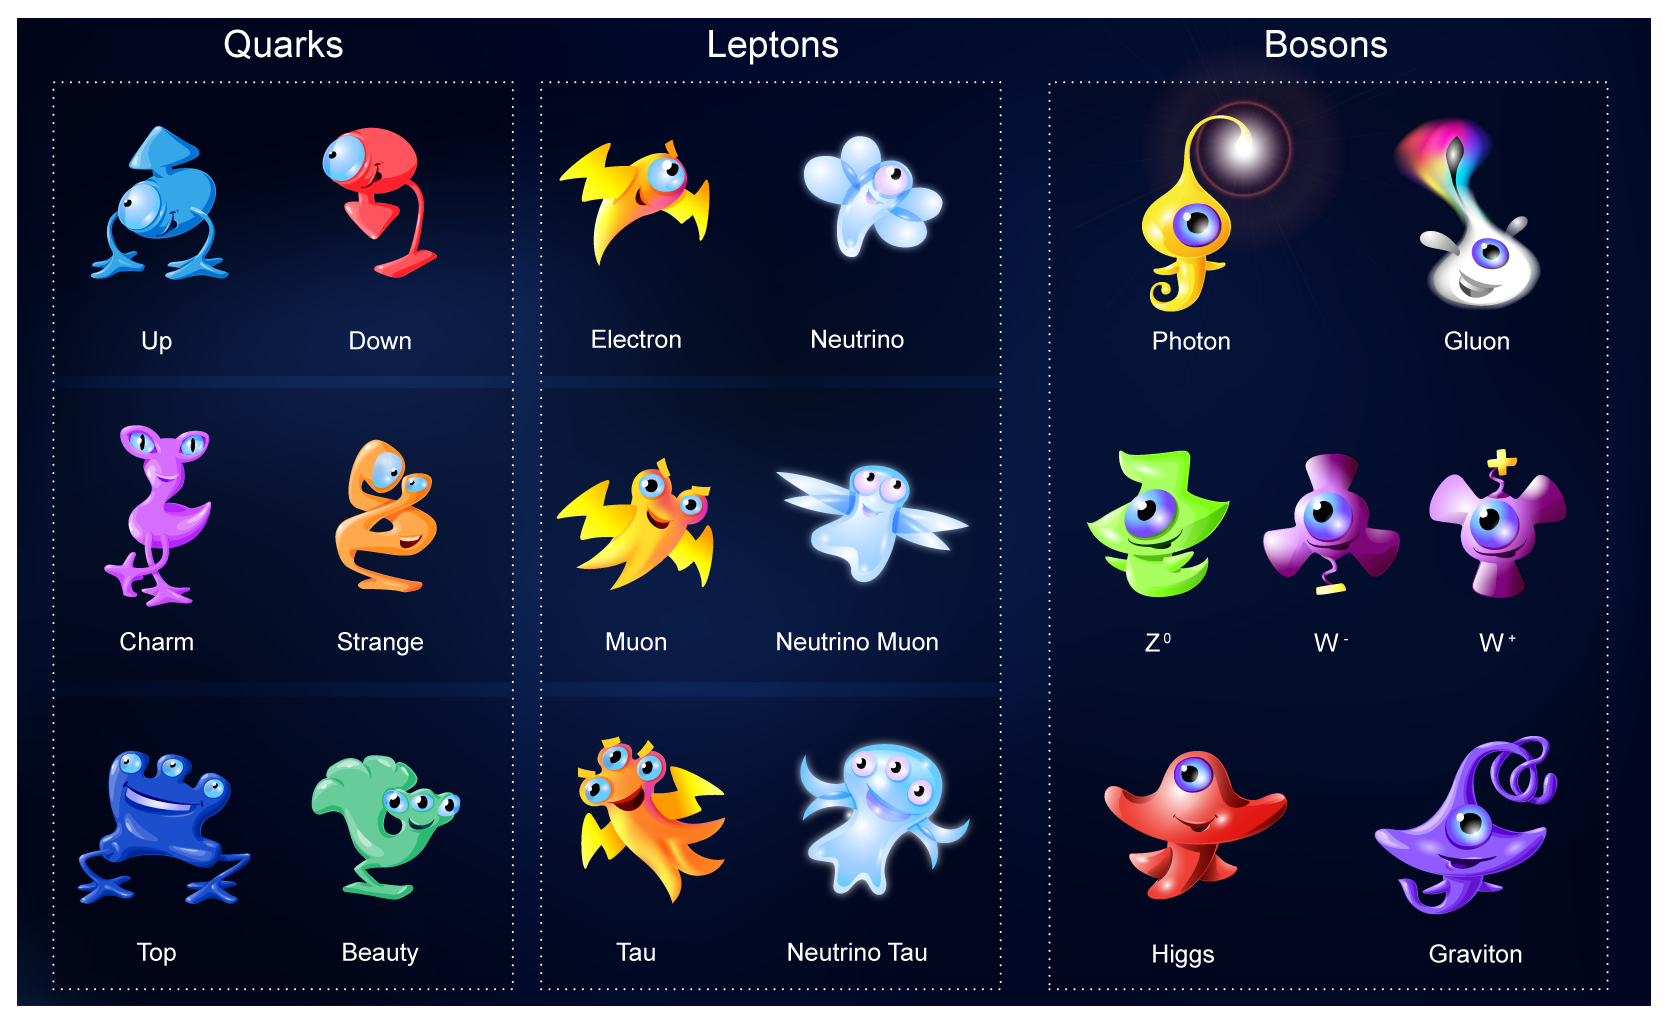
\includegraphics[scale=0.3]{images/particlequest.eps}
\caption{Ejemplo de gamificación: los enemigos en el juego ParticleQuest representan las diferentes partículas subatómicas.
\label{fig:particlequest}}
\end{center}
\end{figure}

La herramienta que se presenta en este trabajo se encuadra dentro de este último tipo de técnicas. La versión gamificada del texto de programa asocia los diferentes elementos del escenario de un videojugo con las instrucciones de código. El dominio de los videojuegos resulta familiar y divertido al usuario. Además, al ser una metáfora basada en agente \cite{travers1996programming} podría asistir también en el diseño de programas concurrentes donde los diferentes hilos de ejecución pueden ser representados por diferentes personajes recorriendo un mismo escenario.


%%%%%%%%%%%%%%%%%%%%%%%%%%%%%  PROPOSAL %%%%%%%%%%%%%%%%%%%%%%%%%%%%%%%%

\section{Propuesta}
\label{sec:proposal}

Seymour Papert, uno de los creadores del lenguaje Logo inventó la
metáfora de la pequeña-persona ({\em little-person}) para explicar a
sus estudiantes cómo funcionaba. La metáfora consiste en que dentro del ordenador viven pequeñas personas (PPs) que son especialistas en
realizar determinadas tareas, y contratan a otras PPs para realizar
subtareas. Las PPs están dormidas normalmente, pero pueden ser
despertadas para que realicen su tarea. Cada vez que una PP necesita
ejecutar una subtarea, contrata una PP especializadad en esa tarea y
se duerme. Cuando la PP contratada termina, vuelve a despertar al
llamador (véase \cite{harvey1985computer}).

Es posible materializar esta metáfora para visualizar a las ``pequeñas personas" realizando su tarea al moverse por las instrucciones de un programa. Para ello, es necesario que tales instrucciones sean visualizadas como diferentes partes del escenario. Atendiendo a la tercera técnica de gamificación mencionada se propone un escenario típico de un videojuego de plataformas. La idea es hacer más atractiva la tarea de codificación y depuración. Quizás el videjouego de este tipo más famoso es Super Mario. Para este trabajo se ha utilizado una versión libre de este juego llamada Secret Maryo Chronicles.

La metáfora utilizada consiste en visualizar un método o una función, como una plataforma en el escenario del videojuego. Todo lo que hay sobre esta plataforma será el contenido del método. El uso de las estructuras de control básicas de un programa se corresponden con otras plataformas o elementos del videojuego por los que el protagonista del videojuego se mueve.  La figura \ref{fig:rules} muestra las reglas de composición utilizadas. Esta analogía resulta muy intuitiva puesto que relaciona la dinámica de ambos contextos. En concreto, para que el flujo de programa pueda ser representado al menos se requieren estos elementos: 

\begin{itemize}
\item {\em Método}: Es representado mediante una plataforma elevada sobre la que se visualizarán . 
\item {\em Condicional}: Es representado mediante una plataforma elevada. Si la condición se cumple, el personaje saltará a la plataforma, si no, pasará por debajo.
\item {\em Switch}: Es representado mediante varias plataformas elevadas apiladas en vertical una para cada caso. El personaje saltará a la plataforma del caso que se cumpla.
\item {\em Bucle}: Es representado mediante una tubería o similar por donde el personaje se introduce y aparece al principio del bucle.
\item {\em Retorno}: Una puerta representa la devolución de datos o salida del método.
\end{itemize}

\begin{figure}[ht]
\begin{center}
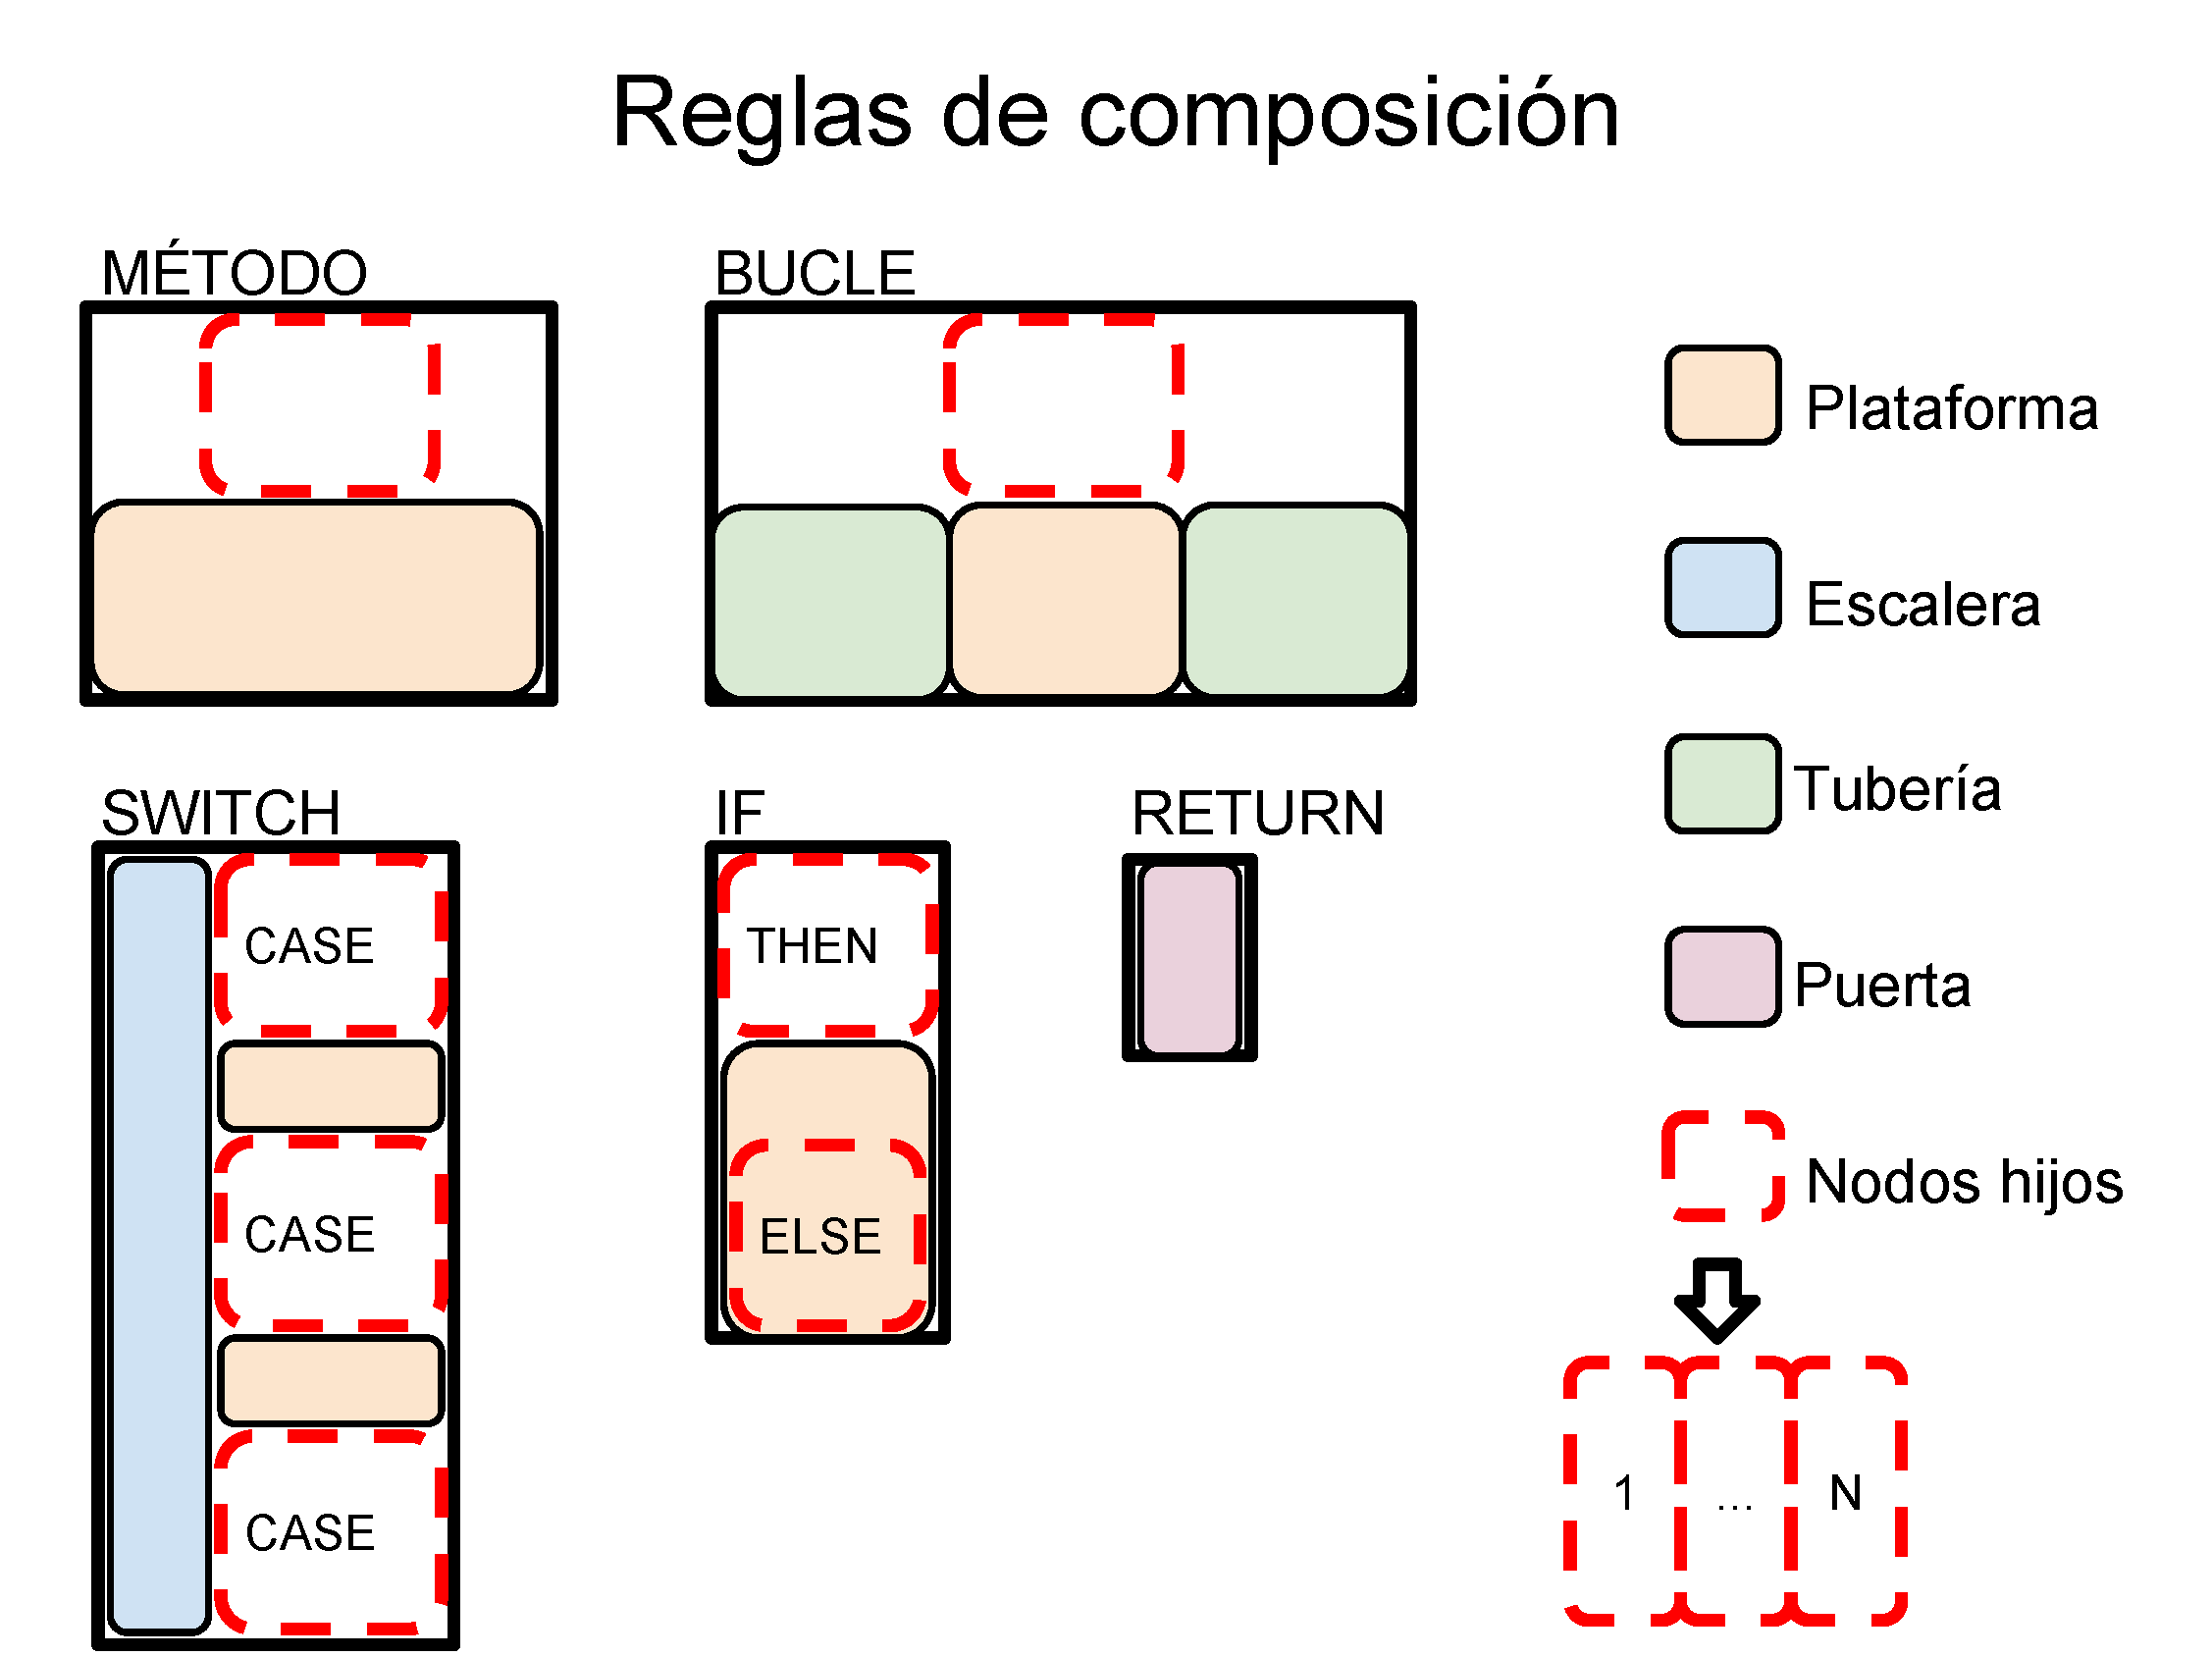
\includegraphics[scale=0.2]{images/nodos.pdf}
\caption{Reglas de composición para los nodos relacionados con el control de flujo de programa.
\label{fig:rules}}
\end{center}
\end{figure}

Existen multitud de videojuegos de plataformas que cumplen con estos requisitos. En este aspecto la visualización puede ser personalizada por el usuario eligiendo los gráficos del videojuego que le resulte más atractivo. Además, otros elementos del lenguaje pueden ser representados mediante diferentes gráficos del juego. Por ejemplo, las expresiones pueden consistir en cajas que el personaje golpea para ver su contenido. Según este esquema el programa de las figuras \ref{fig:flowchart} y \ref{fig:scratch} queda representado en la figura \ref{fig:flowchartgame}.

\begin{figure}[ht]
\begin{center}
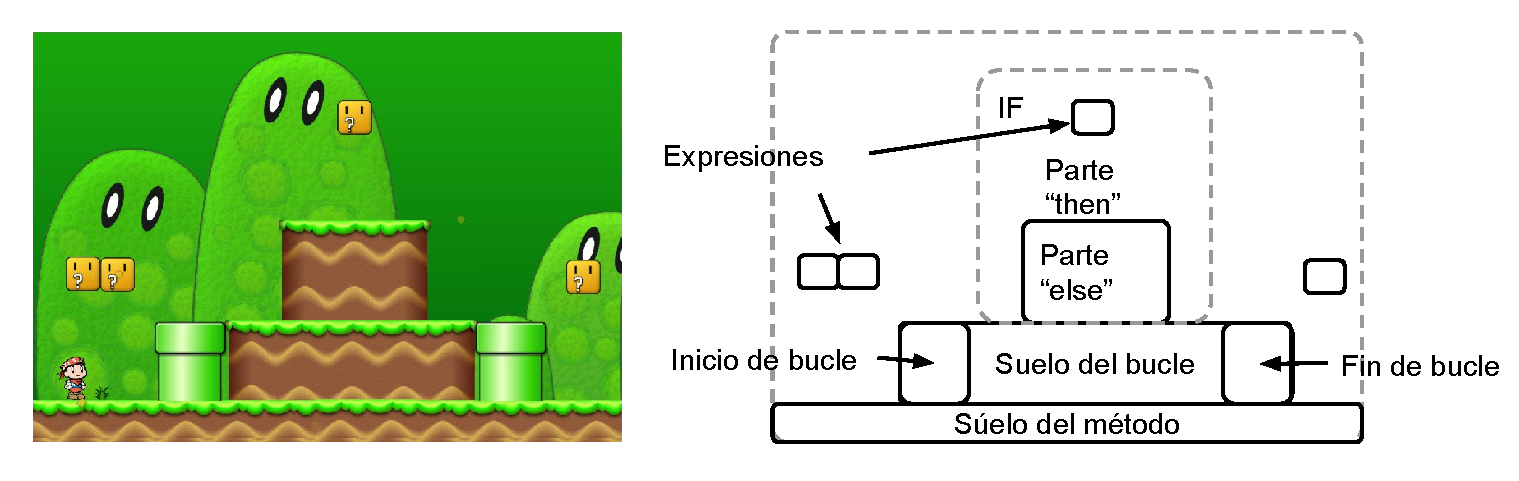
\includegraphics[scale=0.4]{images/flowchartgame2.pdf}
\caption{Visualización propuesta para el programa de ejemplo de la figura \ref{fig:flowchart} y \ref{fig:scratch}. El bucle está representado como la plataforma que hay entre los dos tubos, el IF dentro del bucle es otra plataforma interior y las diferentes expresiones son cajas.
\label{fig:flowchartgame}}
\end{center}
\end{figure}

Para dar más capacidad de expresión y concreción a la representación visual en determinadas zonas del código, existe la posibilidad de elegir diferentes texturas para los elementos del código. Si por ejemplo hay una parte del código más problemática y que por tanto requiere mayor atención, se podrían utilizar gráficos asociados a escenarios más difíciles del videojuego que fueran fácilmente identificables. En la figura \ref{fig:texture} vemos un ejemplo.

\begin{figure}[ht]
\begin{center}
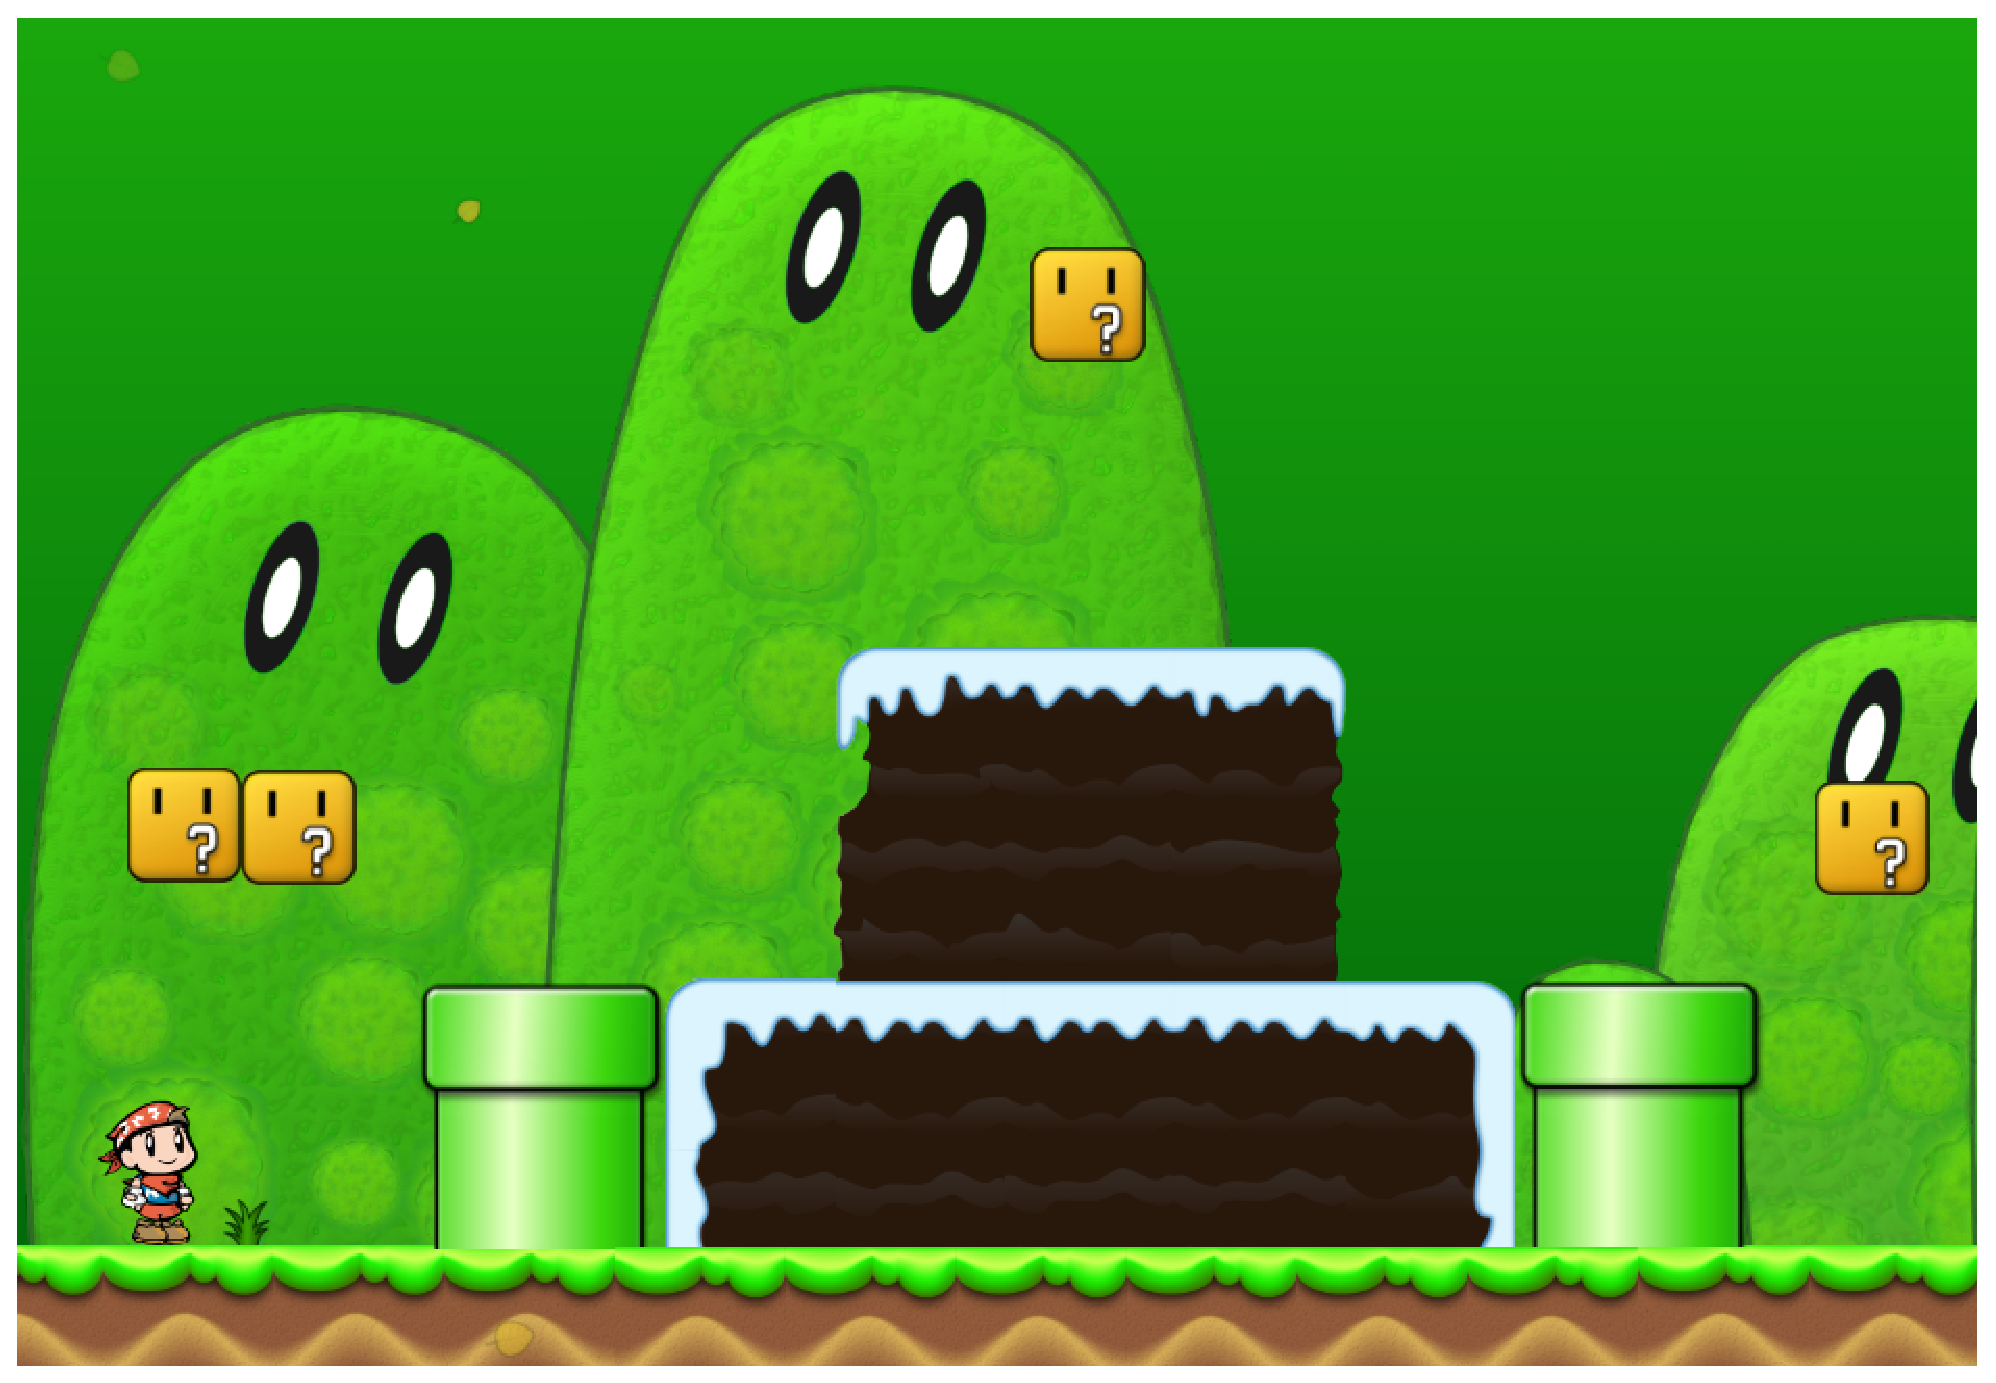
\includegraphics[scale=0.15]{images/texture.eps}
\caption{Visualización donde se ha resaltado todo el código del bucle utilizando plataformas con nieve.
\label{fig:texture}}
\end{center}
\end{figure}

El lenguaje para el que se ha implementado la herramienta de visualización propuesta es Java. El motivo de esta elección es el amplio uso del mismo, y la facilidad que poseen las herramientas de desarrollo para ser extendidas. Además es un lenguaje multiplataforma, gratuito, muy empleado tanto en la docencia, tanto específica de programación como en otras áreas relacionadas en las que se necesitan nociones básicas. Por otro lado es un lenguaje con un gran volumen de nuevos usuarios interesados en aprenderlo cada día gracias en parte al auge de las tecnologías móviles.


%% ANTARES (OK): Deberías hablar también de que es un lenguaje multiplataforma, gratuito, muy empleado en la docencia en multitud de ámbitos (no sólo formación de programadores sino de otros profesionales que adquieren nociones de programación y que suelen ser los que más problemas para ajustarse a los nuevos paradigmas presentan. También comentar que es un lenguaje en auge, con un gran volumen de nuevos usuarios interesados en aprenderlo cada día gracias en parte a las tecnologías móviles.)

%%%%%%%%%%%%%%%%%%%%%%%%%%%%%  DETAILS %%%%%%%%%%%%%%%%%%%%%%%%%%%%%%%%

\section{Implementación}
\label{sec:details}
Para implementar la herramienta de visualización dinámica propuesta se ha utilizado el lenjuaje Java sobre el IDE Eclipse. Eclipse es una plataforma extensible para construir IDEs. Proporciona servicios básicos para utilizar varias herramientas que ayudan en las tareas de programación. Los desarrolladores de herramientas pueden contribuir a la plataforma envolviéndolas en forma de componentes llamados complementos o \emph{plugins}. El mecanismo básico es añadir nuevos elementos de procesamiento a los complementos existentes. Mediante un manifiesto XML se describe la forma en que el entorno de ejecución de Eclipse activará y manejará las instancias del complemento. 

El complemento Progamer consiste en una vista añadida a la perspectiva Java para mostrar la imagen generada a partir del código que se está editando. 

\begin{figure}[ht]
\begin{center}
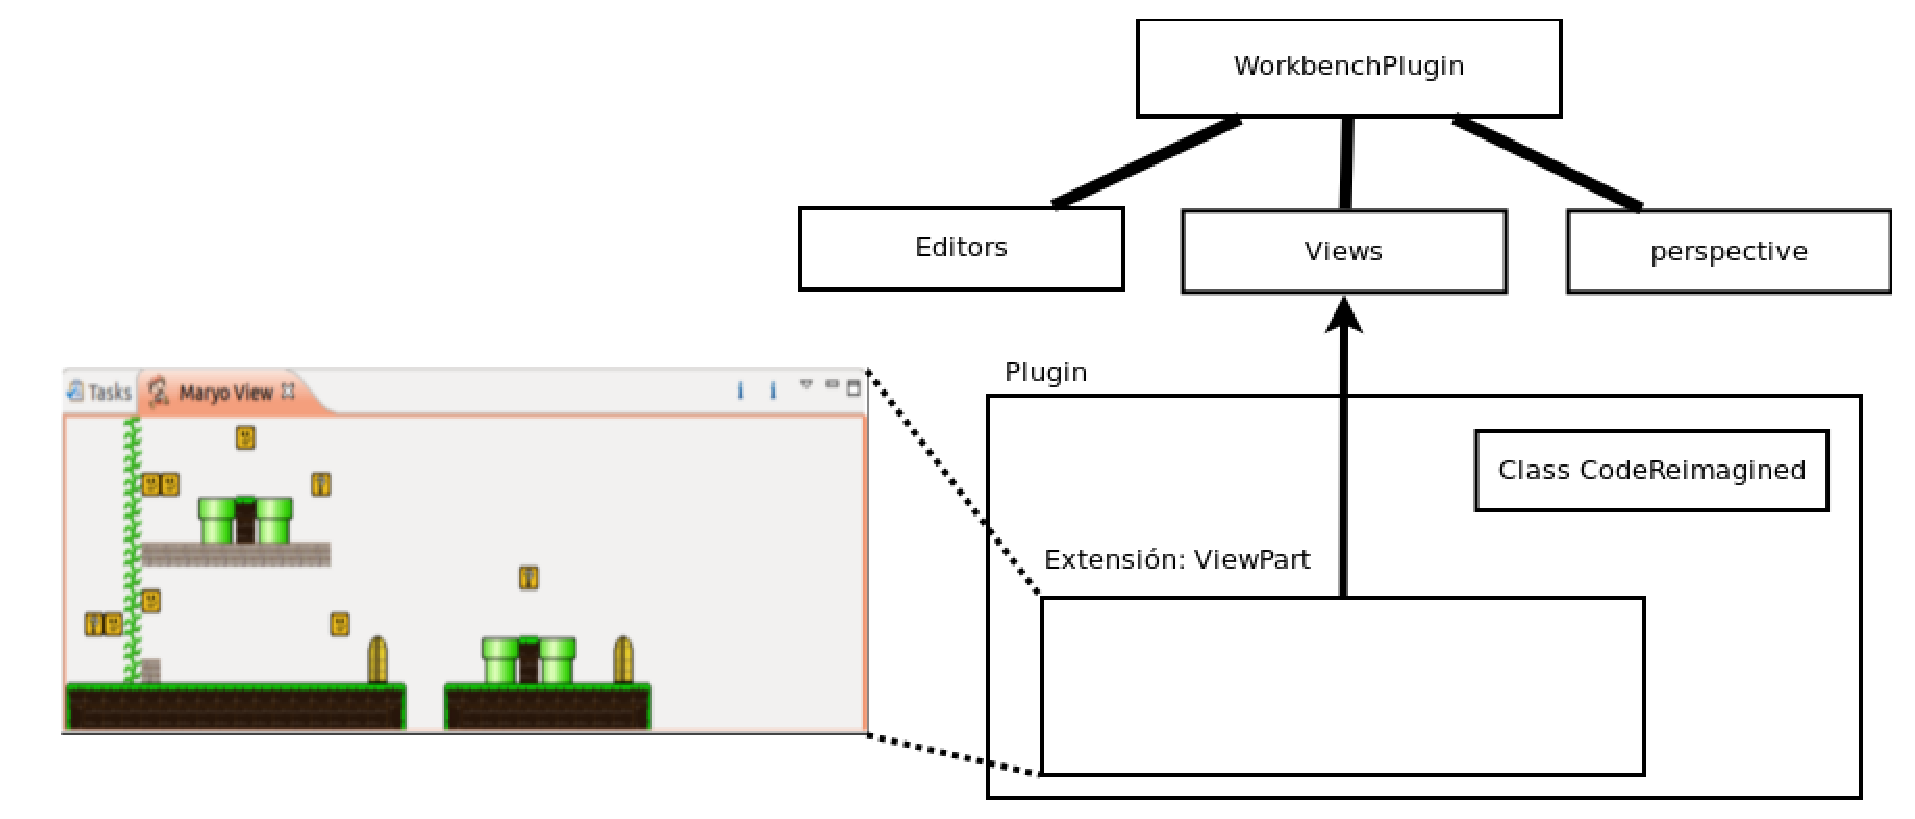
\includegraphics[scale=0.35]{images/crplugin.eps}
\caption{Esquema del complemento como una nueva vista en Eclipse.
\label{fig:crplugin}}
\end{center}
\end{figure}

Para analizar el código se ha usado el patrón \emph{visitor} sobre el árbol sintáctico abstracto del código Java. Recorriendo este árbol se obtiene otro árbol cuyos nodos representan las áreas a dibujar en la vista. Estos objetos nodos heredan de una clase abstracta y especifican la lógica de las reglas de composición de la imagen, es decir, cómo se pintará el elemento de programación dado y qué área resulta de ello. Para generar la imagen en la vista, basta hacer un recorrido de este árbol (sin importar el orden) y llamar al método que dibuja recursivamente el área correspondiente de cada nodo.

\begin{figure}[ht]
\begin{center}
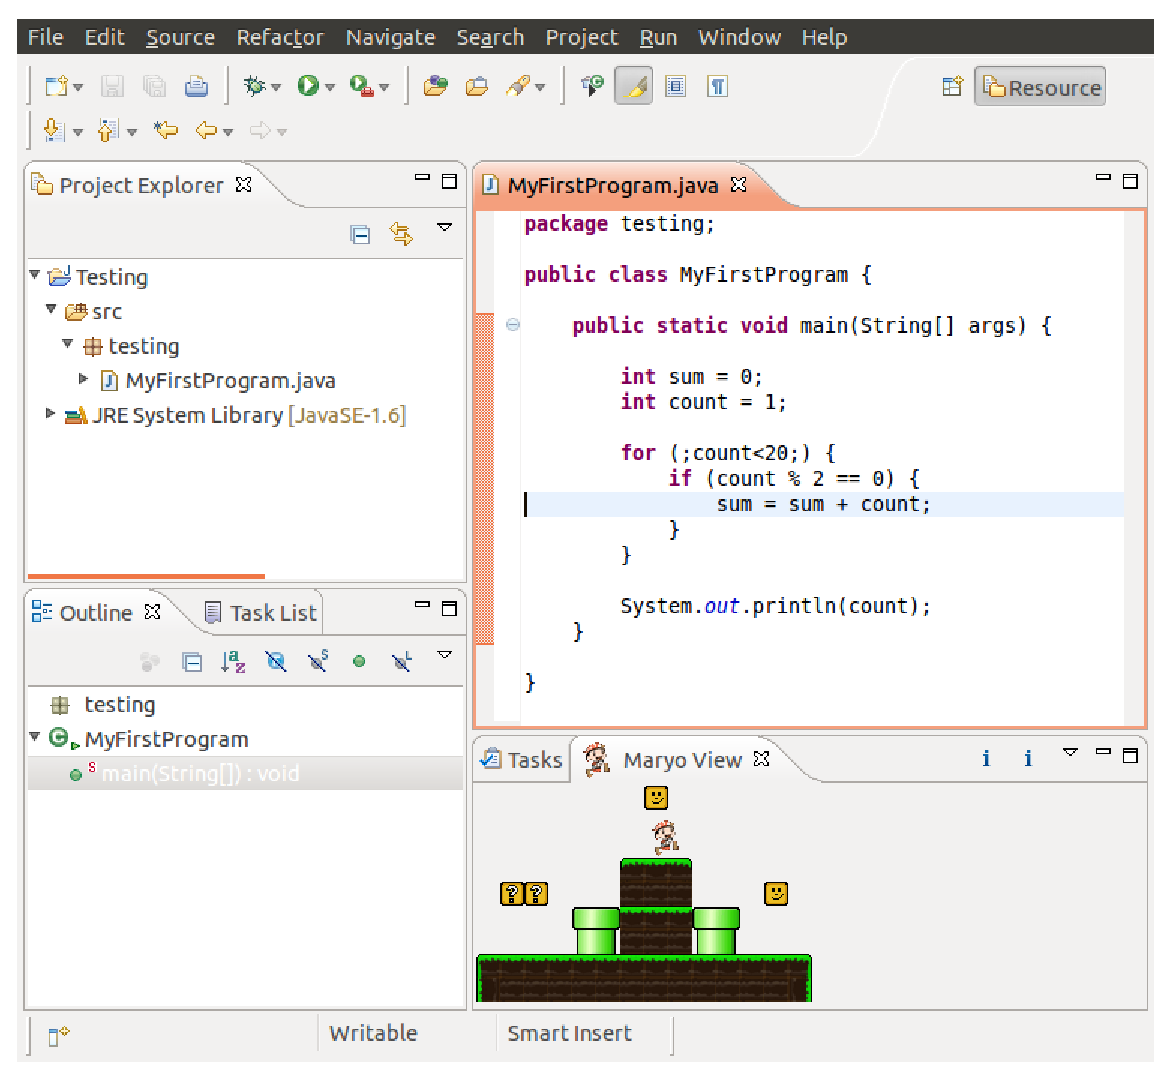
\includegraphics[scale=0.5]{images/eclipse.eps}
\caption{El complemento Progamer muestra el programa de la figura \ref{fig:flowchart} y \ref{fig:scratch} una vez integrado en el entorno Eclipse. El protagonista aparece sobre el área dibujada correspondiente al elemento Java que hay a continuación a partir de la posición actual del cursor.
\label{fig:eclipse}}
\end{center}
\end{figure}

Para representar la dinámica del agente moviéndose sobre la vista se ha
implementado un {\em listener} para el cursor del editor Java, de forma que el personaje aparecerá sobre el área correspondiente al elemento Java que haya inmediatamente después del cursor (figura \ref{fig:eclipse}). Para ello una tabla de dispersión almacena los nodos correspondientes a los elementos Java según su {\em offset} en el archivo de texto.

Otra funcionalidad implementada es la navegación a través del código posicionando el cursor en el editor Java al hacer doble clic sobre el elemento correspondiente de la imagen generada.

Este complemento se presentó al VII Concurso Universitario de Software Libre \footnote{\url{www.concursosoftwarelibre.org}} quedando entre los 10 finalistas a nivel local en la Universidad de Granada. El código está disponible para descarga en \url{https://github.com/javiplay/progamer}.

%ANTARES (OK): Deberías cambiarle el nombre al proyecto.
%ANTARES (pufff ya en otro más pollúo): Echo de menos algún "ejemplo" de equivalentes entre árbol y escenario, ampliando la figura 10 pero quitando "lo que sobra", para hacer mucho más énfasis en la representación. Y usando algún código algo más complejo.

%%%%%%%%%%%%%%%%%%%%%%%%%%%%%  CONCLUSIONS %%%%%%%%%%%%%%%%%%%%%%%%%%%%%%%%

\section{Conclusiones}
\label{sec:conclusions}

En el contexto de la visualización de software y partiendo del concepto de legibilidad del código, este trabajo ha identificado la necesidad de desarrollar técnicas automáticas de visualización de programas, donde la metáfora empleada juegue un papel activo y material tanto para el aprendizaje de los conceptos básicos relacionados con la programación como para la documentación, comprensión, análisis, navegación y evolución del software.

Las metáforas pueden ser concretadas en imágenes compuestas de acuerdo al árbol sintáctico abstracto del programa, donde cada tipo de nodo establece las reglas de composición. Esta técnica habilita el diseño de metáforas específicas para asistir durante el aprendizaje. Las metáforas diseñadas pueden dirigir y concentrar la atención del estudiante asociando los conceptos del dominio de la programación a elementos de otros dominios con los que el estudiante está familiarizado. 

El videojuego de plataformas como dominio fuente para el diseño de la metáfora es adecuado tanto para la representación visual del flujo de control de un programa (mediante el escenario) como para su dinámica o ejecución (mediante la interacción del agente en el escenario). Las sentencias de control son comunes en los lenguajes imperativos y por tanto esta metáfora puede ser implementada para este tipo de lenguajes. 

Una vez concretados los detalles de esta representación, se ha desarrollado una herramienta prototipo de visualización dinámica de código Java en forma de complemento para Eclipse. 

El desarrollo futuro de este trabajo contempla varias líneas:
\begin{itemize}
\item En primer lugar es necesario evaluar la efectividad de esta técnica en la mejora del aprendizaje, comprensión, depuración, navegación y documentación del software mediante diferentes experimentos.
\item Por otro lado sería interesante desarrollar de cara a estos experimentos, juegos serios para abordar los problemas típicos de la asignatura de fundamentos de programación y evaluar así también el potencial de la técnica presentada.
\item De esta forma se continuará con la exploración de nuevas metáforas que destaquen o asistan otros aspectos del lenguaje básicos tales como el uso de expresiones, tipos de datos, variables, llamadas a métodos o uso de parámetros, tanto para docencia como para ingeniería y documentación del software.

\item La metáfora basada en agente, presenta una problemática conocida cuando se utiliza para comprender el funcionamiento de un sistema concurrente. Será interesante comprobar si una visualización activa de ésta pudiera resultar útil al respecto. La idea consiste en que diferentes personajes del videojuego represente distintos hilos de ejecución.
 

%ANTARES (OK): Yo diría que no sólo limitado al ámbito académico "puro" sino incluso a un ámbito más ámplio de la documentación y IS. Además, podrías hablar de lo que has comentado varias veces, del sistema de multiples personajes recorriendo el mapa al mismo tiempo para procesos paralelos o incluso, para ámbitos de procesos concurrentes (muñequitos que van de una "isla a otra" o algo asín)


\item Por último, aunque no relacionado con el ámbito de la educación se planteará el uso de esta técnica para explorar nuevas formas de expresión tecno-artística.
\end{itemize}




%%%%%%%%%%%%%%%%%%%%%%%%%%%%%  ACKNOWLEDGEMENTS %%%%%%%%%%%%%%%%%%%%%%%%%%%%%%%%

\section*{Agradecimientos}
Este trabajo ha sido apoyado por el proyecto SIPEsCa con
referencia G-GI3000/IDIF, el proyecto Anyself
con referencia TIN2011-28627-C04-02 del Ministerio de Innovación y
Ciencia y el proyecto 83, CANUBE, concedido por el CEI-BioTIC de la
Universidad de Granada. 

\bibliographystyle{splncs}


\bibliography{bibliography}


\end{document}

%%Está chulo el trabajo, el STATE OF ART es de premio :)
